\documentclass[../main.tex]{subfiles}

\begin{document}
    Testowanie oparte na \textbf{strukturze} oprogramowania lub systemu, np.:

    \begin{tabular}{p{4cm} || p{12cm}}
        \textbf{Poziom testów} & \textbf{Przykład struktury}\\
        \hline
        \hline
        \textbf{testy modułowe} & kod: instrukcje, decyzje, rozgałęzienia, ścieżki\\
        \hline
        \textbf{testy integracyjne} & drzewo wywołań\\
        \hline
        \textbf{testy systemowe} & struktura menu, proces biznesowy, struktura strony www\\
    \end{tabular}


    Przykładowe metody \textbf{wizualizacji} struktury:
    \begin{itemize}
        \item \textbf{graf przepływu sterowania} (CFG, Control Flow Graph) lub danych
        \item \textbf{model procesu biznesowego} w BPML
        \item \textbf{diagram aktywności} (czynności) w UML
    \end{itemize}
    W technikach białoskrzynkowych przypadki testowe projektuje się tak, by
    pokrywały określone elementy modelu (krawędzie, decyzje, ścieżki itp.)

    Pokrycie (dla metod białoskrzynkowych) sprawdza jakość testów czarnoskrzynkowych; następnie techniki
    białoskrzynkowe dostarczają testów w celu zwiększenia tego pokrycia

    \begin{figure}[H]
        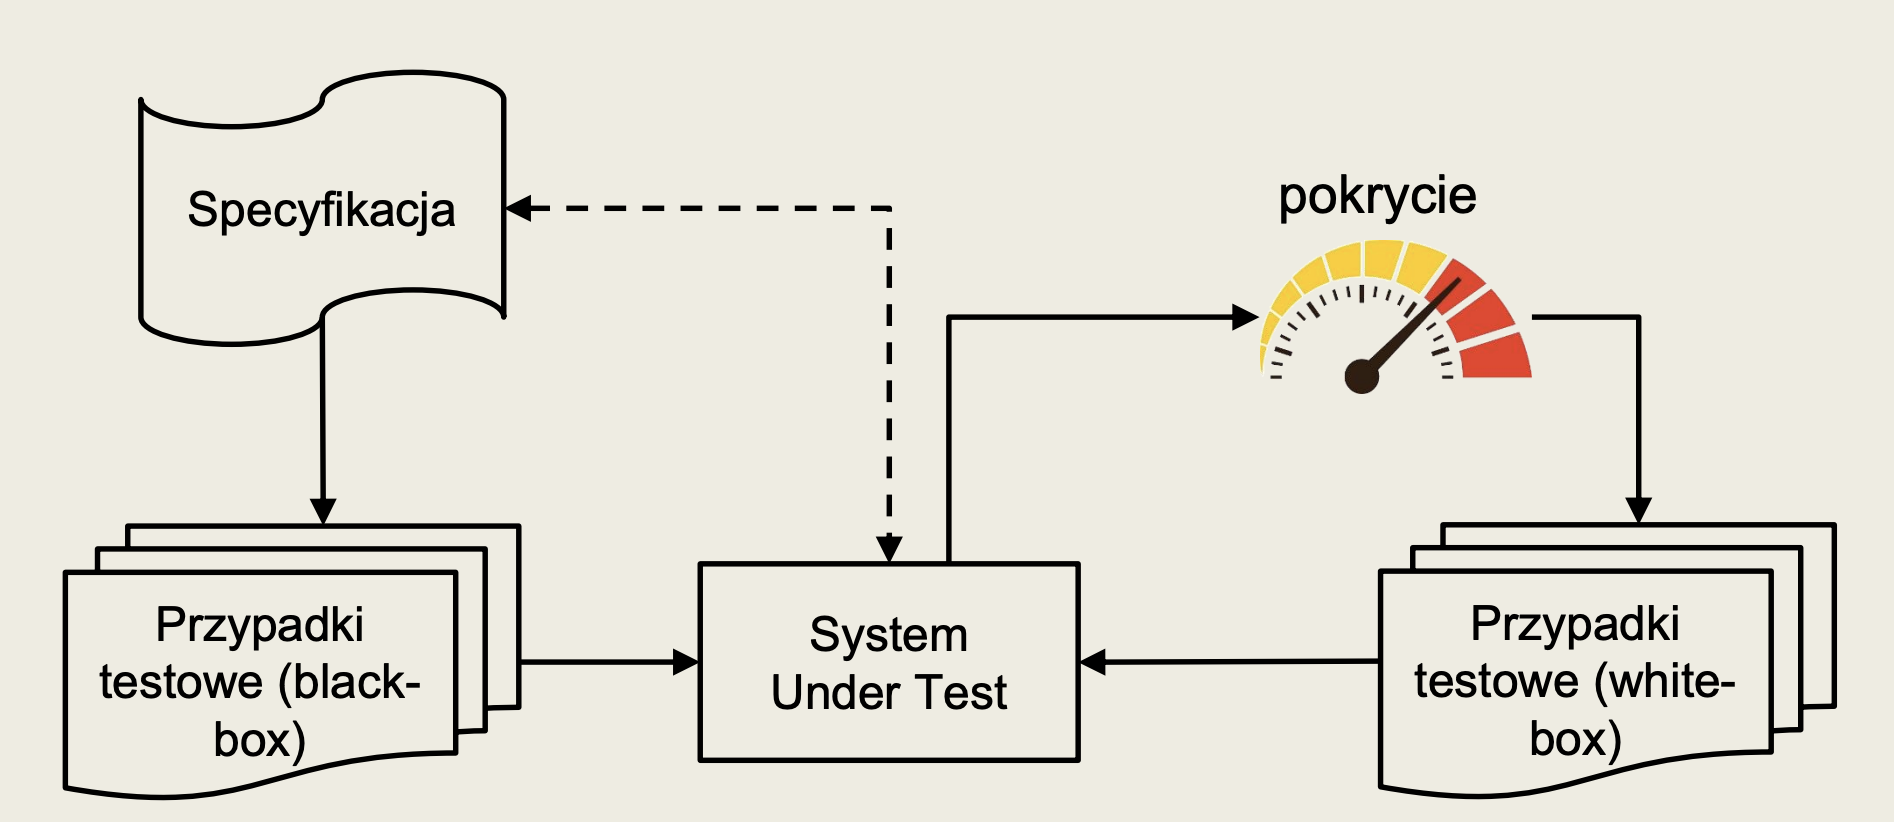
\includegraphics[width=\linewidth]{whitebox.png}
    \end{figure}


    \subsection{Pokrycia grafowe}

    \begin{table}[H]
        \begin{center}
            \begin{tabular}{p{8cm} | p{8cm}}
                \multicolumn{2}{c}{\textbf{POKRYCIA}}\\
                \hline
                \textbf{Syntaktyczne} & "teoretyczne", wszystkie ścieżki grafu ignorując logikę poszczególnych węzłów.\\
                \hline
                \textbf{Semantyczne} & uwzględniające tę logikę.\\

            \end{tabular}
        \end{center}
    \end{table}

    \begin{table}[H]
        \begin{center}
            \begin{tabular}{p{8cm} | p{8cm}}
                \textbf{Graf przepływu sterowania} &  \textbf{Graf przepływu danych}\\
                \hline
                \hline
                \begin{itemize}
                    \item \textbf{CFG} - Control Flow Graph
                    \item graficzna reprezentacja przepływu sterowania (graf skierowany)
                    \begin{itemize}
                        \item wierzchołki = bloki bazowe
                        \item krawędzie = przejścia między blokami
                    \end{itemize}
                    \item blok bazowy = sekwencja instrukcji taka, że jeśli wykona się
                    pierwsza z nich, wszystkie pozostałe w obrębie bloku wykonają się również
                \end{itemize}
                &
                \begin{itemize}
                    \item oparty na grafie przepływ sterowania
                    \item zawiera informacje o operacjach na zmiennych
                    \item możliwe operacje:
                    \begin{itemize}
                        \item \textbf{d} (definition, definicja) – miejsce definiowania zmiennej
                        \item \textbf{u} (use, użycie) – miejsce użycia zmiennej
                        \item \textbf{k} (kill, zabicie) – miejsce usunięcia zmiennej z pamięci
                    \end{itemize}
                \end{itemize}

                Dla każdego węzła $B$ definiujemy zbiory $d(B)$, $u(B)$, $k(B)$ zawierające zmienne definiowane, używane lub
                zabijane w danym węźle.
                \\
            \end{tabular}
        \end{center}
    \end{table}



    \subsubsection{Pokrycie instrukcyjne}
    \begin{table}[H]
        \begin{center}
            \begin{tabular}{p{8cm} p{8cm}}
                \textbf{Cechy:} & \textbf{ Problemy praktyczne:}\\
                \begin{itemize}
                    \item elementy pokrycia: \textbf{instrukcje} kodu
                    \item kryterium pokrycia instrukcyjnego: każda linia kodu jest wykonana
                    przynajmniej raz w jakimś teście
                    \item osiągnięcie 100\% pokrycia jest często \textbf{nieosiągalne}
                \end{itemize}
                &
                \begin{itemize}
                    \item jak definiować linię kodu? (linia fizyczna? wykonywalna?)
                    \item czy rozważać pojedyncze instrukcje, czy bloki bazowe?
                    \begin{itemize}
                        \item to wpływa na metryki pokrycia
                    \end{itemize}
                \end{itemize}
            \end{tabular}
        \end{center}
    \end{table}




    \subsubsection{Pokrycie krawędziowe (branch testing)}
    \begin{itemize}
        \item inna nazwa: \textbf{pokrycie przejść} między instrukcjami
        \item z punktu widzenia struktury, wymagane jest przejście po każdej
        \textbf{krawędzi CFG}, czyli testowany jest każdy \textbf{przepływ sterowania}
        \item \textbf{suita testowa spełniająca 100\% pokrycia instrukcji nie musi
        spełniać 100\% przejść między instrukcjami!}
        \item Przy założeniu, że CFG ma co najmniej 1 krawędź, \textbf{pokrycie
        krawędziowe subsumuje pokrycie instrukcyjne, nie na odwrót}.
    \end{itemize}


    \subsubsection{Pełne pokrycie ścieżek}
    \begin{table}[H]
        \begin{center}
            \begin{tabular}{p{8cm} p{8cm}}
                \begin{itemize}
                    \item możliwe, gdy \textbf{nie ma pętli} lub \textbf{liczba iteracji} wszystkich pętli jest \textbf{ograniczona} z góry (rozsądną wartością)
                    \item najczęstszy przypadek: \textbf{diagramy przepływu procesów}
                    \item nawet dla kodu bez pętli liczba wszystkich ścieżek może \textbf{rosnąć wykładniczo} względem punktów decyzyjnych
                    \item \textbf{zbiór ścieżek liniowo niezależnych} to odpowiednik \textbf{bazy przestrzeni wektorowej}.
                    \item \textbf{złożoność cyklomatyczna CFG} - liczba ścieżek liniowo niezależnych.
                \end{itemize}
                &
                \begin{itemize}
                    \item \textbf{algorytm wyznaczania ścieżek liniowo niezależnych}
                    \begin{itemize}
                        \item wychodzimy od prostej ścieżki
                        \item jedna decyzja zmieniana w porównaniu z poprzednią ścieżką
                        \item po zmianie, będąc w węźle już kiedyś odwiedzonym, kontynuujemy wędrówkę wzdłuż tamtej ścieżki,
                        (staramy się zmienić tak mało, jak to możliwe, w porównaniu z poprzednimi ścieżkami)
                        \item zwykle pętle iterujemy max. raz
                    \end{itemize}
                \end{itemize}
            \end{tabular}
        \end{center}
    \end{table}


    \subsubsection{Pokrycie przepływu danych}
    Wierzchołki: p,n; Zmienne: v.
    \begin{table}[H]
        \begin{center}
            \begin{tabular}{p{8cm} p{8cm}}
                \textbf{Kryteria pokrycia przepływu danych:}
                \begin{itemize}
                    \item \textbf{All-defs}: $\forall n : v \in def(n)$
                    zbiór testów zawiera przynajmniej jedną du-ścieżkę ze zbioru $du(n, v)$
                    \item \textbf{All-uses}: $\forall (n, m) : v \in def(n)$ and $v \in use(m)$ zbiór testów zawiera przynajmniej jedną
                    du-ścieżkę ze zbioru $du(n, m, v)$
                    \item \textbf{All-du-paths}: $\forall n \forall v: v \in def(n)$
                    zbiór testów zawiera wszystkie du-ścieżki ze zbioru $du(n, v)$
                \end{itemize}
                &
                Ścieżka $p = (p_1 , \dots, p_n)$ jest \textbf{def-czysta} ze względu na zmienną v, jeśli v nie jest
                definiowana w żadnym węźle ścieżki poza $p_1$.

                Ścieżka $p = (p_1 , \dots, p_n)$ jest \textbf{du-ścieżką} ze względu na zmienną v, jeśli:
                \begin{enumerate}
                    \item jest def-czysta ze względu na v
                    \item $v \in def(p_1)$
                    \item $v \in use(p_n)$
                \end{enumerate}

                $du(n, v)$ - zbiór wszystkich du-ścieżek ze względu na v rozpoczynających się w n

                $du(n, m, v)$ - zbiór wszystkich du-ścieżek ze względu na v rozpoczynających się w n i kończących w m
            \end{tabular}
        \end{center}
    \end{table}


    \subsubsection{Pokrycie pętli}

    \begin{table}[H]
        \begin{center}
            \begin{tabular}{| p{8cm} | p{8cm} |}
                \hline
                \multicolumn{2}{|c|}{\textbf{RODZAJE PĘTLI}}\\
                \hline
                \hline
                \textbf{proste} & \textbf{zagnieżdżone}\\
                \hline
                \begin{itemize}
                    \item przetestuj brak wykonania pętli (pominięcie pętli, wykonanie 0 razy)
                    \item przetestuj pojedyncze wykonanie pętli
                    \item przetestuj podwójne wykonanie pętli
                    \item przetestuj typową liczbę wykonań pętli
                    \item przetestuj max-1, max, max+1 wykonań pętli, gdzie max =
                    maksymalna dopuszczalna liczba iteracji
                \end{itemize}
                &
                \begin{itemize}
                    \item dla najbardziej zagnieżdżonej pętli przeprowadź test pętli prostej
                    \item powtórz ten test dla kolejnych coraz bardziej zewnętrznych pętli
                    \item powtarzaj, dopóki nie przetestujesz najbardziej zewnętrznej
                \end{itemize}\\
                \hline
                \hline
                \textbf{połączone} & \textbf{nieustrukturalizowane}\\
                \hline
                \begin{itemize}
                    \item jeśli pętle połączone są niezależne, dla każdej z nich wykonaj test pętli prostej
                    \item jeśli pętle połączone są zależne, przetestuj je jak zagnieżdżone
                \end{itemize}
                &
                \begin{itemize}
                    \item najlepsze wyjście: refaktoryzacja
                    kodu w celu usunięcia
                    nieustrukturyzowanych pętli
                    \item pozbycie się instrukcji goto
                \end{itemize}\\
                \hline
            \end{tabular}
        \end{center}
    \end{table}

    \begin{table}[H]
        \begin{center}
            \begin{tabular}{ p{8cm}  p{8cm} }
                \textbf{Co testujemy w przypadku pętli?}
                \begin{itemize}
                    \item problemy w \textbf{inicjalizowaniu} pętli (np. „błąd o jeden” w iteratorze)
                    \item problemy z niezainicjalizowanymi zmiennymi (poprzez jednokrotne
                    wykonanie pętli)
                    \item problemy z \textbf{powtarzaniem instrukcji} zawartych w pętli
                    \item kwestie związane z \textbf{wydajnością}/zasobami
                \end{itemize}
                &
                \textbf{Problemy z testowaniem pętli}
                \begin{itemize}
                    \item istnienie pętli = \textbf{nieskończona liczba ścieżek} do przetestowania
                    \item pętle zagnieżdżone = jeszcze większy problem
                    \item defekty w pętlach są często \textbf{trudne do wykrycia}
                    \item jak testować pętle? istnieją różne kryteria i podejścia
                \end{itemize}
            \end{tabular}
        \end{center}
    \end{table}
\end{document}